\begin{frame}[nofoottext]{Equation System Structure}
    \centering
    \begin{columns}
        \begin{column}{0.5\linewidth}
            \begin{itemize}
                \item Non-linear equation system.
                \item Sparse symmetrical gradient matrix.
                \item Block structure regarding quantities (state variables, fluxes) and constraints (with their lambdas).
            \end{itemize}
        \end{column}
        \begin{column}{0.5\linewidth}
            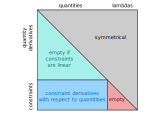
\includegraphics[width=\textwidth]{img/implementation/sparse_structure}
        \end{column}
    \end{columns}
\end{frame}
